\graphicspath{{Figures/}}

\title{\fontsize{33}{45}{\huge Pattern Classification\newline{\large Lecture 06: Linear Discriminant Functions}\newline \vspace{8pt} \Large \vspace{-1.1cm}}}

\vspace{0.5cm}
\author{\vspace{0.4cm}\\\large{\bf Kundan Kumar\\\url{https://github.com/erkundanec/PatternClassification}}
%Associate Professor\\Department of ECE}
}
% - Give the names in the same order as the appear in the paper.
% - Use the \inst{?} command only if the authors have different
%   affiliation.
%\vspace{1cm}
\institute[Indian Institute of Technology Kharagpur] % (optional, but mostly needed)
{
\vspace{1.8cm}
%\includegraphics[height=.17\textheight]{SOAlogo.png}\\
% Faculty of Engineering (ITER)\\ S`O'A Deemed to be University, Bhubaneswar, India-751030\\


 \copyright\  2020 Kundan Kumar, All Rights Reserved\\
  \vspace{-1.1cm}}
% - Use the \inst command only if there are several affiliations.
% - Keep it simple, no one is interested in your street address.
\date{}
% To remove page number from a perticular slide
{
\setbeamertemplate{logo}{}
\makeatletter
\setbeamertemplate{footline}{
        \leavevmode%
  
  % First line.
  \hbox{%
  \begin{beamercolorbox}[wd=.2\paperwidth,ht=\beamer@decolines@lineup,dp=0pt]{}%
  \end{beamercolorbox}%
  \begin{beamercolorbox}[wd=.8\paperwidth,ht=\beamer@decolines@lineup,dp=0pt]{lineup}%
  \end{beamercolorbox}%
  } %
  % Second line.
  \hbox{%
  \begin{beamercolorbox}[wd=\paperwidth,ht=\beamer@decolines@linemid,dp=0pt]{linemid}%
  \end{beamercolorbox}%
  } %
  % Third line.
  \hbox{%
  \begin{beamercolorbox}[wd=.1\paperwidth,ht=\beamer@decolines@linebottom,dp=0pt]{}%
  \end{beamercolorbox}%
  \begin{beamercolorbox}[wd=.9\paperwidth,ht=\beamer@decolines@linebottom,dp=0pt]{linebottom}%
  \end{beamercolorbox}%
  }%
        }
\makeatother
\begin{frame}
\titlepage
\end{frame}
}

\section{Linear Discriminant Functions}
\subsection{}
\begin{frame}{}
\begin{variableblock}{\centering \Large \textbf{\vspace{4pt}\newline Linear Discriminant Functions\vspace{4pt}}}{bg=slidecolor,fg=white}{bg=slidecolor,fg=white}
\end{variableblock}
\end{frame}

\begin{frame}{Introduction}
\begin{itemize}
\item In parametric estimation, we assumed that the forms for the underlying {\color{mycolor1}probability densities were known}, and used the training samples to estimate the values of their parameters.
\item Instead, assume that the proper forms for the discriminant
functions is known, and use the samples to estimate the values of parameters of the classifier.
\item None of the various procedures for determining discriminant functions require
knowledge of the forms of underlying probability distributions so called {\color{mycolor2}nonparametric} approach.
\item Linear discriminant functions are relatively {\color{mycolor1}easy to compute} and estimate the form using training samples.
\end{itemize}
\end{frame}

\begin{frame}{Linear discriminant functions and decisions surfaces}
\begin{itemize}
\item A {\color{mycolor1}discriminant function} is a linear combination of the components of ${\rm x}$ can be written as
\begin{equation}
g({\rm x})={\rm w}^T{\rm x}+w_0 \nonumber
\end{equation}
where ${\rm w}$ is the {\color{mycolor2}weight vector} and $w_0$ the {\color{mycolor4}bias} or {\color{mycolor4}threshold} weight.
\item The equation $g({\rm x}) = 0$ defines the {\color{mycolor1}decision surface} that separates points from different classes.
\item Linear discriminant functions are going to be studied for 
\begin{itemize}
\item two-category case,
\item multi-category case, and
\item general case
\end{itemize} 
For the general case
there will be $c$ such discriminant functions, one for each of $c$ categories.\nocite{duda2012pattern}
%\item A two-category classifier with a discriminant function of the form (1) uses the following rule:\\
%	Decide $w_1$ if $g(x) > 0$ and $w_2$ if $g(x) < 0$\\
%	Decide $w_1$ if ${\rm w}^tx > -w_0$ and $w_2$ otherwise\\
%	If $g(x) = 0$ then $x$ is assigned to either class
\end{itemize}
\end{frame}

\section{Two-category}
\subsection{}
\begin{frame}{Two-Category Case}
\begin{itemize}
\setlength{\itemsep}{12pt}
\item A two-category classifier with a discriminant function of the form $g({\rm x})={\rm w}^T{\rm x}+w_0$ uses the following rule:\\
\begin{equation}
{\sf Decide}~~~~\left\{ {\begin{array}{*{20}{c}}
{{\omega_1}}&{{\sf if}~g({\rm x}) > 0}\\
{{\omega_2}}&{\rm otherwise}
\end{array}} \right.\nonumber
\end{equation}
\item Thus, ${\rm x}$ is assigned to $\omega_1$ if the {\color{mycolor2}inner product} ${\rm w}^T{\rm x}$ exceeds the
threshold $-w_0$ and to $\omega_2$ otherwise.
\item If $g({\rm x})=0$, ${\rm x}$ can ordinarily be assigned to either class, or can be left undefined.
%\begin{equation}
%{\sf Decide}~~~~\left\{ {\begin{array}{*{20}{c}}
%{{\omega_1}}&{{\sf if}~g({\rm x}) \geq 0}\\
%{{\omega_2}}&{\rm otherwise}
%\end{array}} \right.\nonumber
%\end{equation}
\end{itemize}
\end{frame}

\begin{frame}{A simple linear classifier}
\begin{figure}
\includegraphics[scale=0.93]{Ch0501}
\caption{A simple linear classifier having $d$ input units, each corresponding to the values of the components of an input vector. Each input feature value $x_i$ is multiplied by its corresponding weight $w_i$; the output unit sums all these products and emits $+1$ if ${\rm w}^T{\rm x}+w_0>0$ or $-1$ otherwise}
\end{figure}
\end{frame}

\begin{frame}{Two-Category Case}
\begin{itemize}
\item The equation $g({\rm x}) = 0$ defines the decision surface that separates points assigned to the category ${\omega_1}$ from points assigned to the category ${\omega}_2$
\item When $g({\rm x})$ is linear, the decision surface is a hyperplane.
%\item Algebraic measure of the distance from ${\rm x}$ to the hyperplane (interesting result!)
\item If ${\rm x}_1$ and ${\rm x}_2$ are both on the decision
surface, then
\begin{align}
{\rm w}^T{\rm x}_1+w_0={\rm w}^T{\rm x}_2+w_0~~~~~~~~~~~~~~~~~~~~~~~~~~~ \nonumber\\
\Rightarrow ~~~~{\rm w}^T({\rm x}_1-{\rm x}_2)=0~~~~~~~~~~~~~~~~~~~~~~~~~~~~~~~~~\nonumber
\end{align}
\vspace{1cm}
\item This shows that ${\rm w}$ is normal to any vector lying in the hyperplane.
\end{itemize}
\begin{tikzpicture}[remember picture,overlay]
  \node (img1) at (11,2.8) {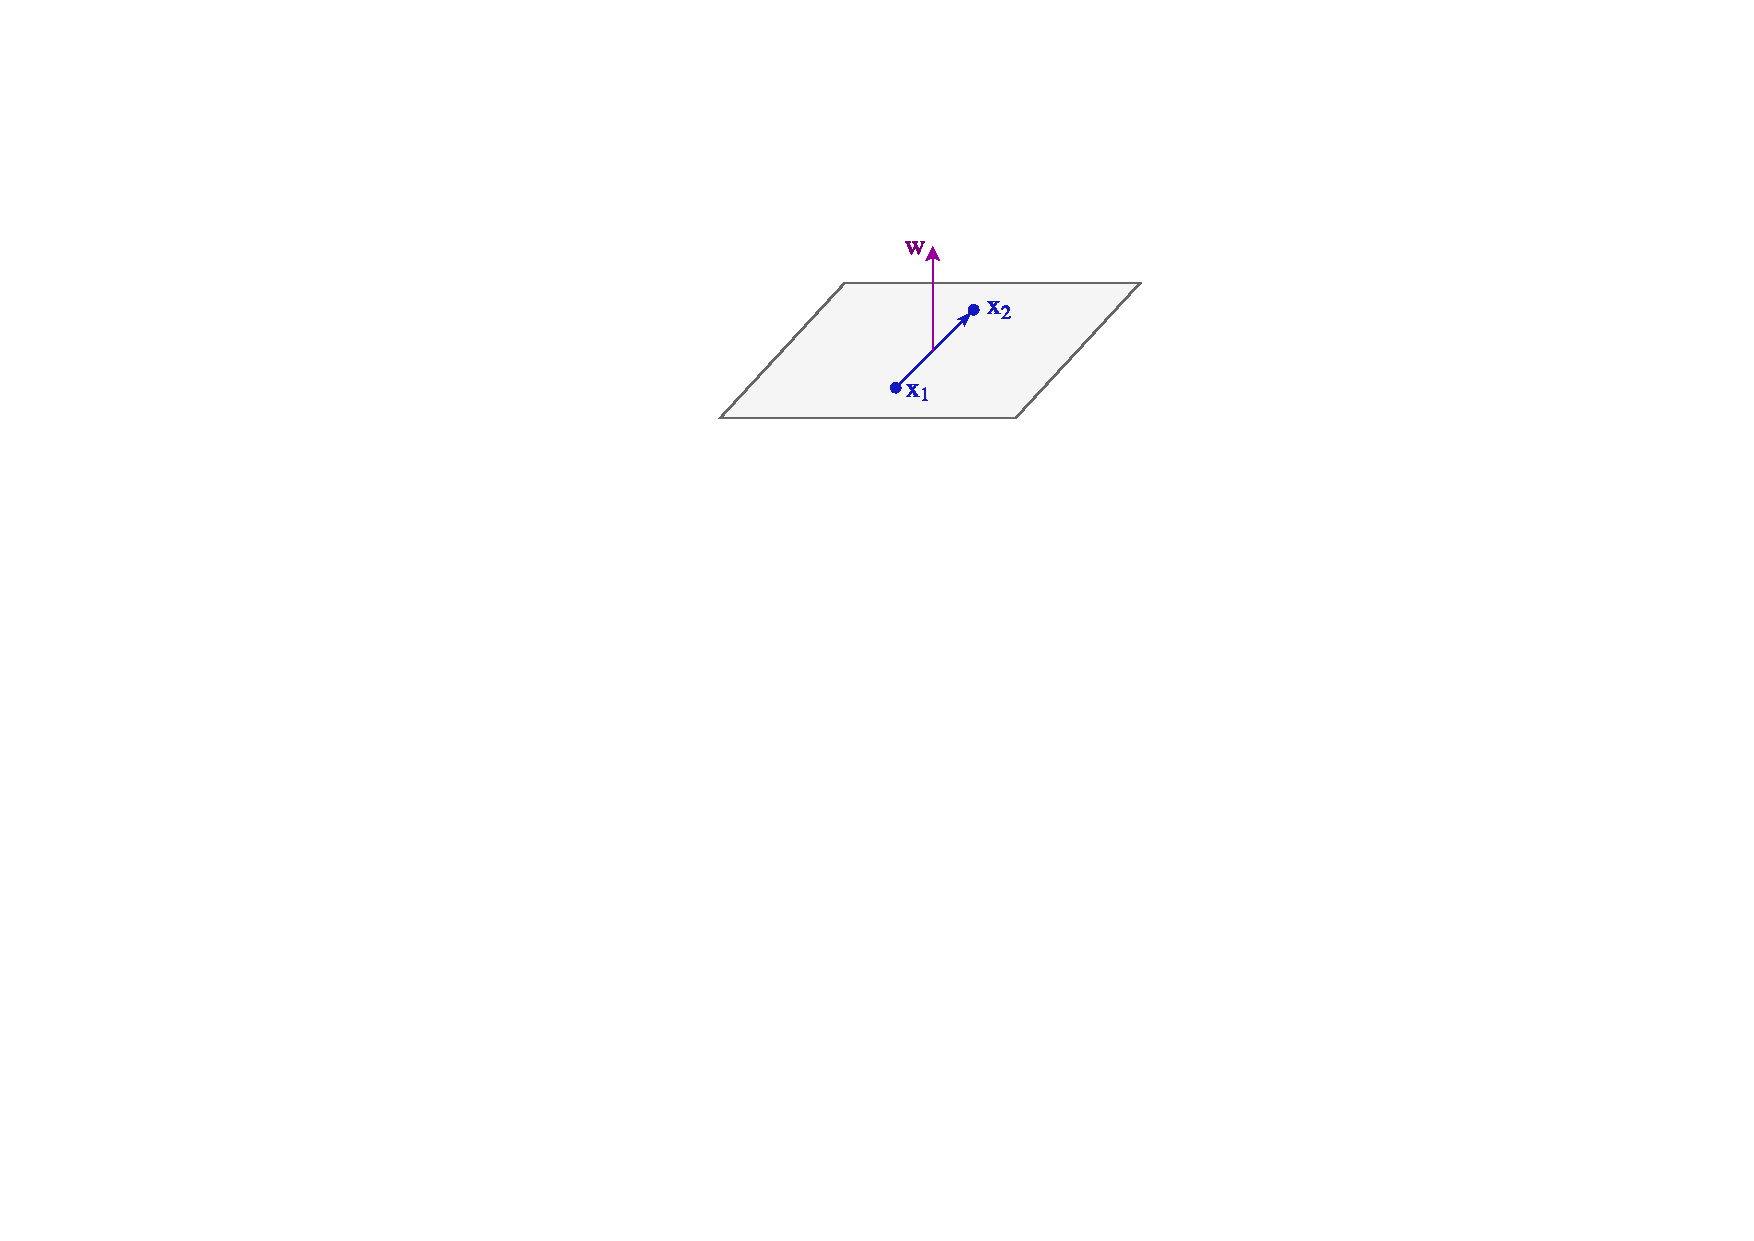
\includegraphics[height=2.6cm]{LDF001}};
\end{tikzpicture}
\end{frame}

\begin{frame}{Two-Category Case}
\begin{itemize}
\item The discriminant function $g({\rm x})$ gives an algebraic measure of the distance from $\rm x$ to the hyperplane. The easiest way to see this is to express ${\rm x}$ as
\begin{equation}
{\rm x} = {{\rm x}_p} + r\frac{{\rm w}}{{\left\| {\rm w} \right\|}} \nonumber
\end{equation}
\end{itemize}
\begin{columns}
\begin{column}{8.5cm}
\begin{itemize}
\item where ${\rm x}_p$ is the normal projection of ${\rm x}$ onto $H$, and $r$ is the desired algebraic distance which is positive if ${\rm x}$ is on the positive side and negative if ${\rm x}$ is on the negative side.
\item Because, $g({\rm x}_p)=0$
\begin{equation}
r = \frac{{g({\rm x})}}{{\left\| {\rm w} \right\|}}~~~~~~~~~~~~~~~~~~ \nonumber
\end{equation}
\end{itemize}
\end{column}
\begin{column}{4.5cm}
%\vspace{-1cm}
%\begin{figure}
%\includegraphics[scale=1.05]{Ch0502}
%\end{figure}
\end{column}
\end{columns}
\begin{tikzpicture}[remember picture,overlay]
  \node (img1) at (12,2.8) {\includegraphics[height=5.6cm]{Ch0502}};
\end{tikzpicture}
\end{frame}

\begin{frame}{Two-Category Case}
\begin{columns}
\begin{column}{6cm}
\begin{itemize}
\item The distance from the origin to $H$ is given by $\frac{w_0}{||{\rm w}||}$. 
\vspace{10pt}
\item If $w_0>0$, the origin is on the positive side of $H$, and if $w_0<0$, it is on the negative side.
\vspace{10pt}
\item If $w_0 = 0$, then $g({\rm x})$ has the homogeneous form ${\rm w}^T{\rm x}$, and the hyperplane passes through the
origin.
\end{itemize}
\end{column}
\begin{column}{7.5cm}
\vspace{-6pt}
\begin{figure}
\includegraphics[scale=1]{Ch0502}
\caption{The linear decision boundary $H$, where $g(x)={\rm w}^T{\rm x}+w_0$, separates the feature space into two half-spaces $\mathcal{R}_1$ (where $g({\rm  x})>0$) and $\mathcal{R}_2$ (where $g({\rm x})<0)$)}
\end{figure}
\end{column}
\end{columns}
\end{frame}

\begin{frame}{Two-Category Case}
\begin{itemize}
\item In conclusion, a linear discriminant function divides the feature space by a hyperplane decision surface.
\item The orientation of the surface is determined by the normal vector ${\rm w}$ and the location of the surface is determined by the bias $w_0$.
\item The discriminant function $g({\rm x})$ is proportional to the signed distance from ${\rm x}$ to the hyperplane, with $g({\rm x})>0$ when ${\rm x}$ is on the positive side, and $g({\rm x})<0$ when ${\rm x}$ is on the negative side.
\end{itemize}
\end{frame}

\section{Multi-category}
\subsection{}
\begin{frame}{Multi-category case}
\begin{itemize}
\item There is more than one way to devise multi-category classifiers employing linear discriminant functions.
\begin{columns}
\begin{column}{4cm}
\begin{itemize}
\item c two-class problem ({\color{mycolor1}one-vs-rest})
\end{itemize}
\begin{figure}
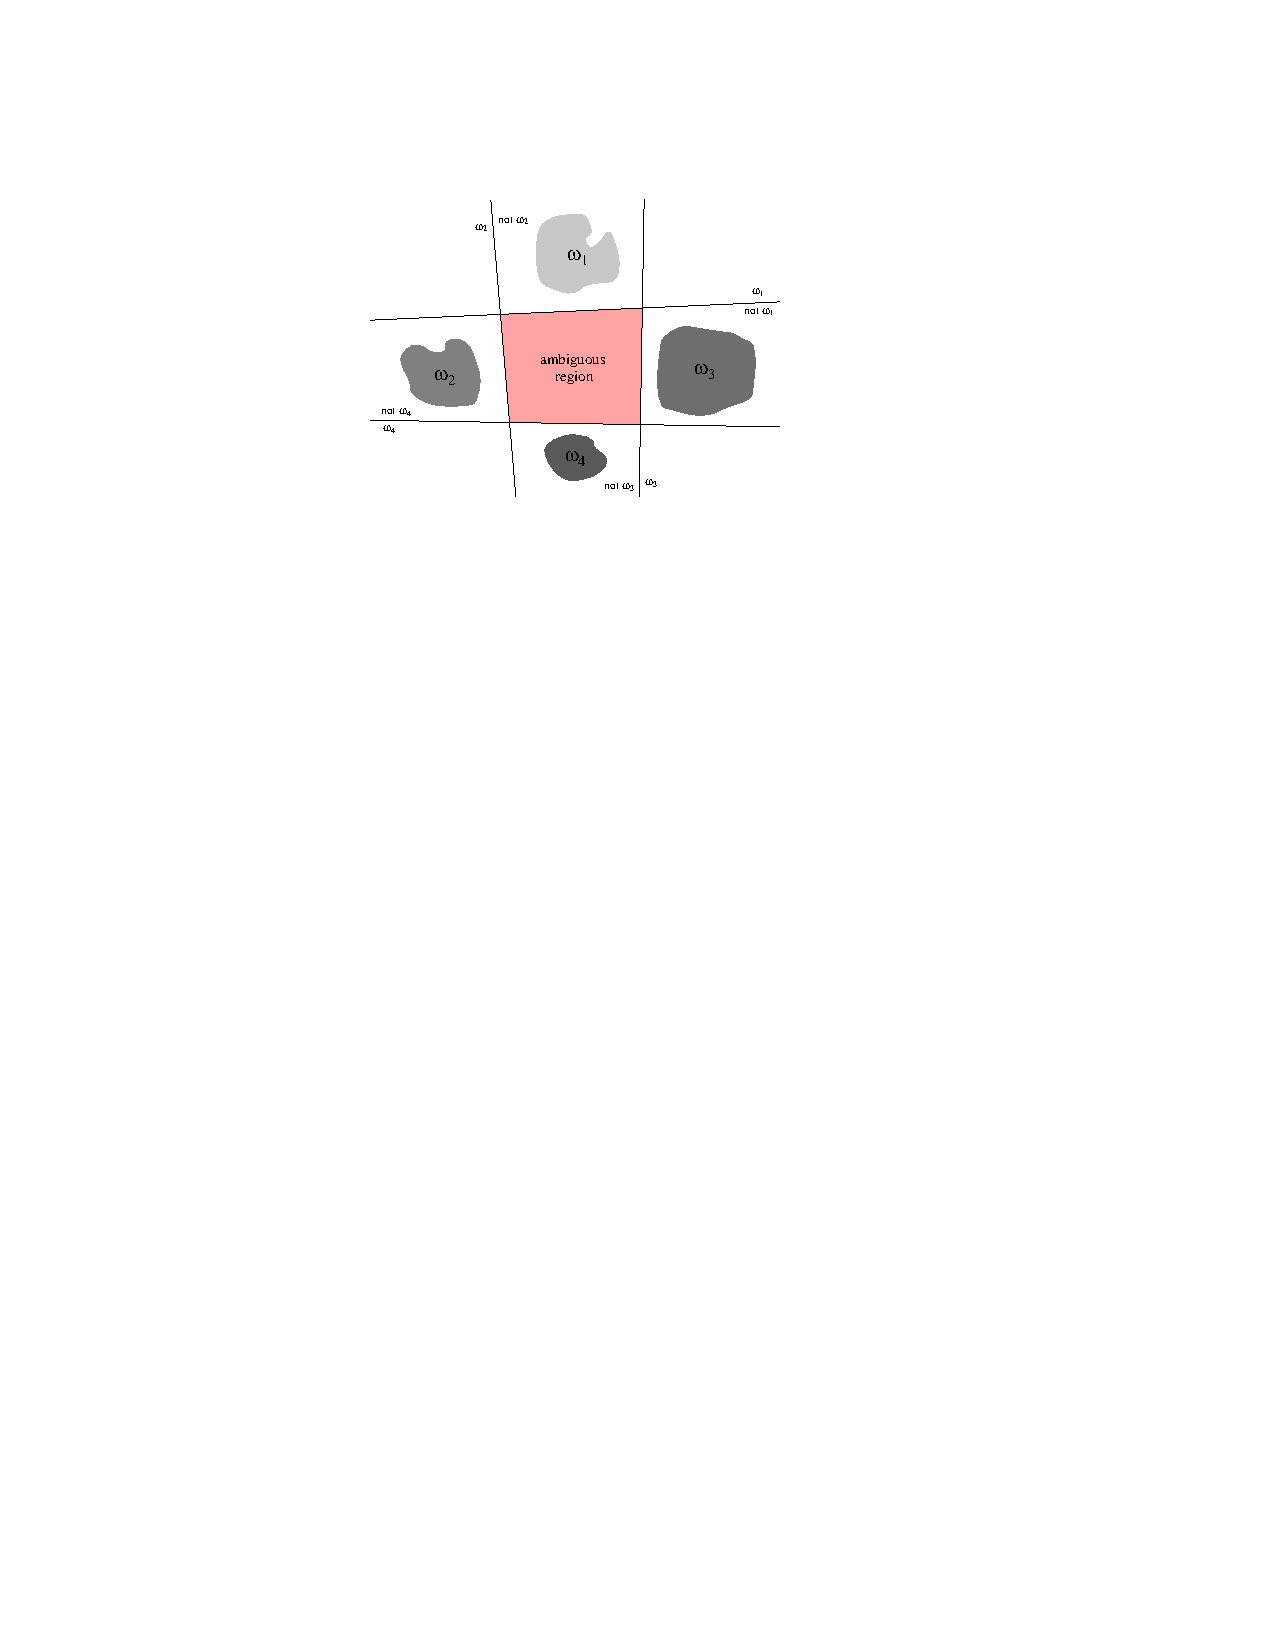
\includegraphics[scale=0.65]{ldf01}
\end{figure}
\end{column}
\begin{column}{5cm}
\begin{itemize}
\item $c(c-1)/2$ linear discriminants, one for every pair of classes ({\color{mycolor1}one-vs-one}).
\end{itemize}
\begin{figure}
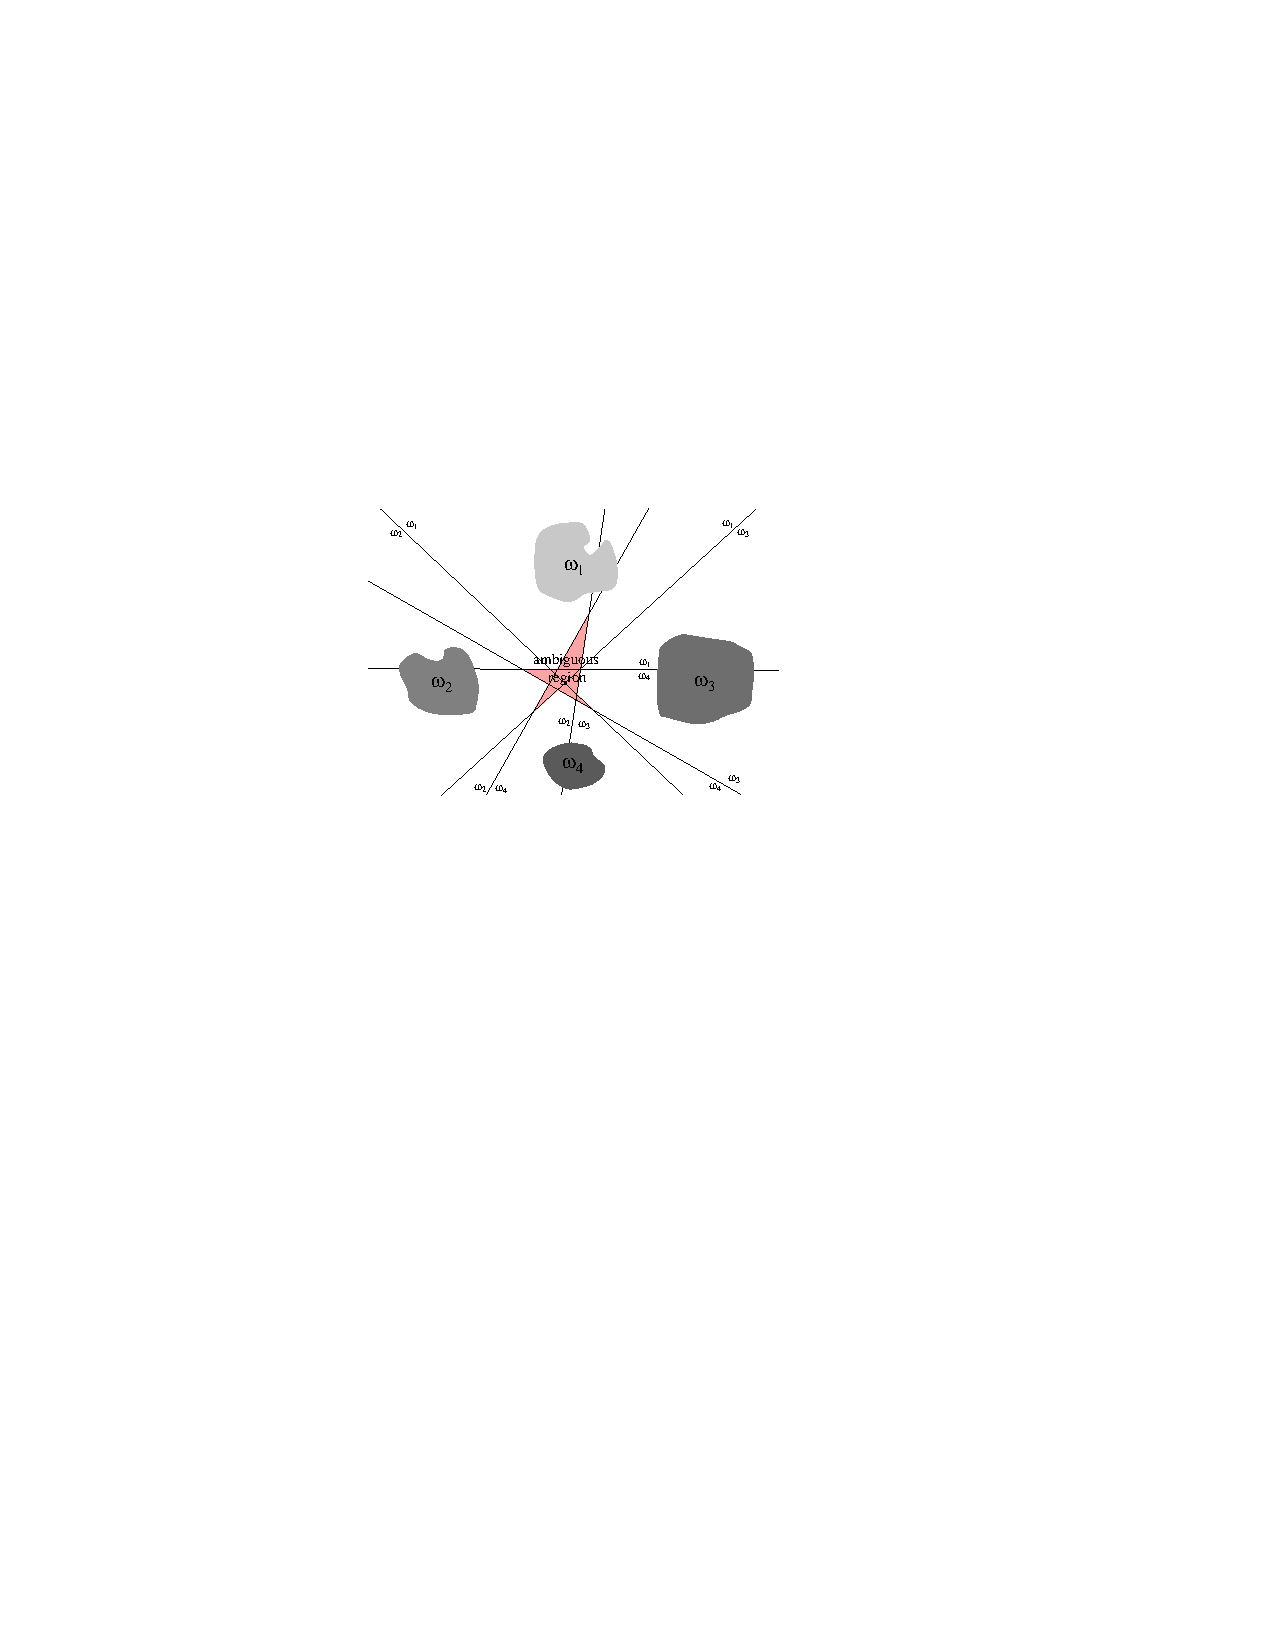
\includegraphics[scale=0.65]{ldf02}
\end{figure}
\end{column}
\end{columns}

\item Pink regions have ambiguous category assignment.
\end{itemize}
\end{frame}

\begin{frame}{Multi-category case}
\begin{itemize}
\item More effective way is to define $c$ linear discriminant functions
\begin{equation}
g_i({\rm x})={\rm w}^T_i{\rm x}+w_{i0}~~~~i=1,2,\ldots,c \nonumber
\end{equation}
	and assign ${\rm x}$ to $\omega_i$ if $g_i({\rm x}) > g_j({\rm x})$ for all $j\neq i$; in case of ties, the classification is undefined
\item In this case, resulting classifier is a ``\textit{\color{mycolor2}linear machine}''.
\item A linear machine divides the feature space into $c$ decision regions, with $g_i({\rm x})$ being the largest discriminant if ${\rm x}$ is in the region $\mathcal{R}_i$.
\item For a two contiguous regions $\mathcal{R}_i$ and $\mathcal{R}_j$; the boundary that separates them is a portion of hyperplane $H_{ij}$ defined by:
\begin{equation}
g_i({\rm x})=g_j({\rm x})~~~~~or~~~~~({\rm w}_i-{\rm w}_j)^T{\rm x}+(w_{i0}-w_{j0})=0 \nonumber
\end{equation}
\end{itemize}
\end{frame}

\begin{frame}{Multi-category case}
\begin{itemize}
\item It follows at once that ${\rm w}_i-{\rm w}_j$ is normal to $H_{ij}$, and the signed distance from ${\rm x}$ to $H_{ij}$ is given by 
\begin{equation}
r = \frac{{({g_i}({\rm x}) - {g_j}({\rm x}))}}{{\left\| {{{\rm w}_i} - {{\rm w}_j}} \right\|}} \nonumber
\end{equation}
\end{itemize}
\begin{figure}
\includegraphics[scale=0.7]{Ch0503}
\caption{Decision boundaries produced by a linear machine for a three-class problem and a five-class problem}
\end{figure}
\end{frame}



%\begin{frame}{The Two-Category Case}
%\begin{itemize}
%\item For the two-category case, the decision rule can be written as
%\begin{equation}
%{\sf Decide}~~~~\left\{ {\begin{array}{*{20}{c}}
%{{\omega_1}}&{{\sf if}~g({\rm x})>0}\\
%{{\omega_2}}&{\sf otherwise~~~~~~~}
%\end{array}} \right.\nonumber
%\end{equation}
%\item The equation $g({\rm x}) = 0$ defines the decision boundary that separates points assigned to $\omega_1$ from points assigned to $\omega_2$.
%\item When $g({\rm x})$ is linear, the decision surface is a hyperplane whose orientation is determined by the normal vector ${\rm w}$ and location is determined by the bias $w_0$.
%\end{itemize}
%\end{frame}

%\begin{frame}{The Multicategory Case}
%\begin{itemize}
%\item There is more than one way to devise multicategory classifiers using linear discriminant functions.
%\item For example, we can reduce the problem as $c$ two-class problems, where the $i$th problem is solved by a linear discriminant that separates points assigned to $\omega_i$ from those not assigned to $\omega_i$.
%\item Alternatively, we can use $c(c-1)/2$ linear discriminants, one for every pair of classes.
%\item Also, we can use $c$ linear discriminants, one for each class, and assign $x$ to $\omega_i$
%if $g_i({\rm x}) > g_j ({\rm x})$ for all $j\neq i$.
%\end{itemize}
%\end{frame}

%\begin{frame}{The Multicategory Case}
%\begin{figure}
%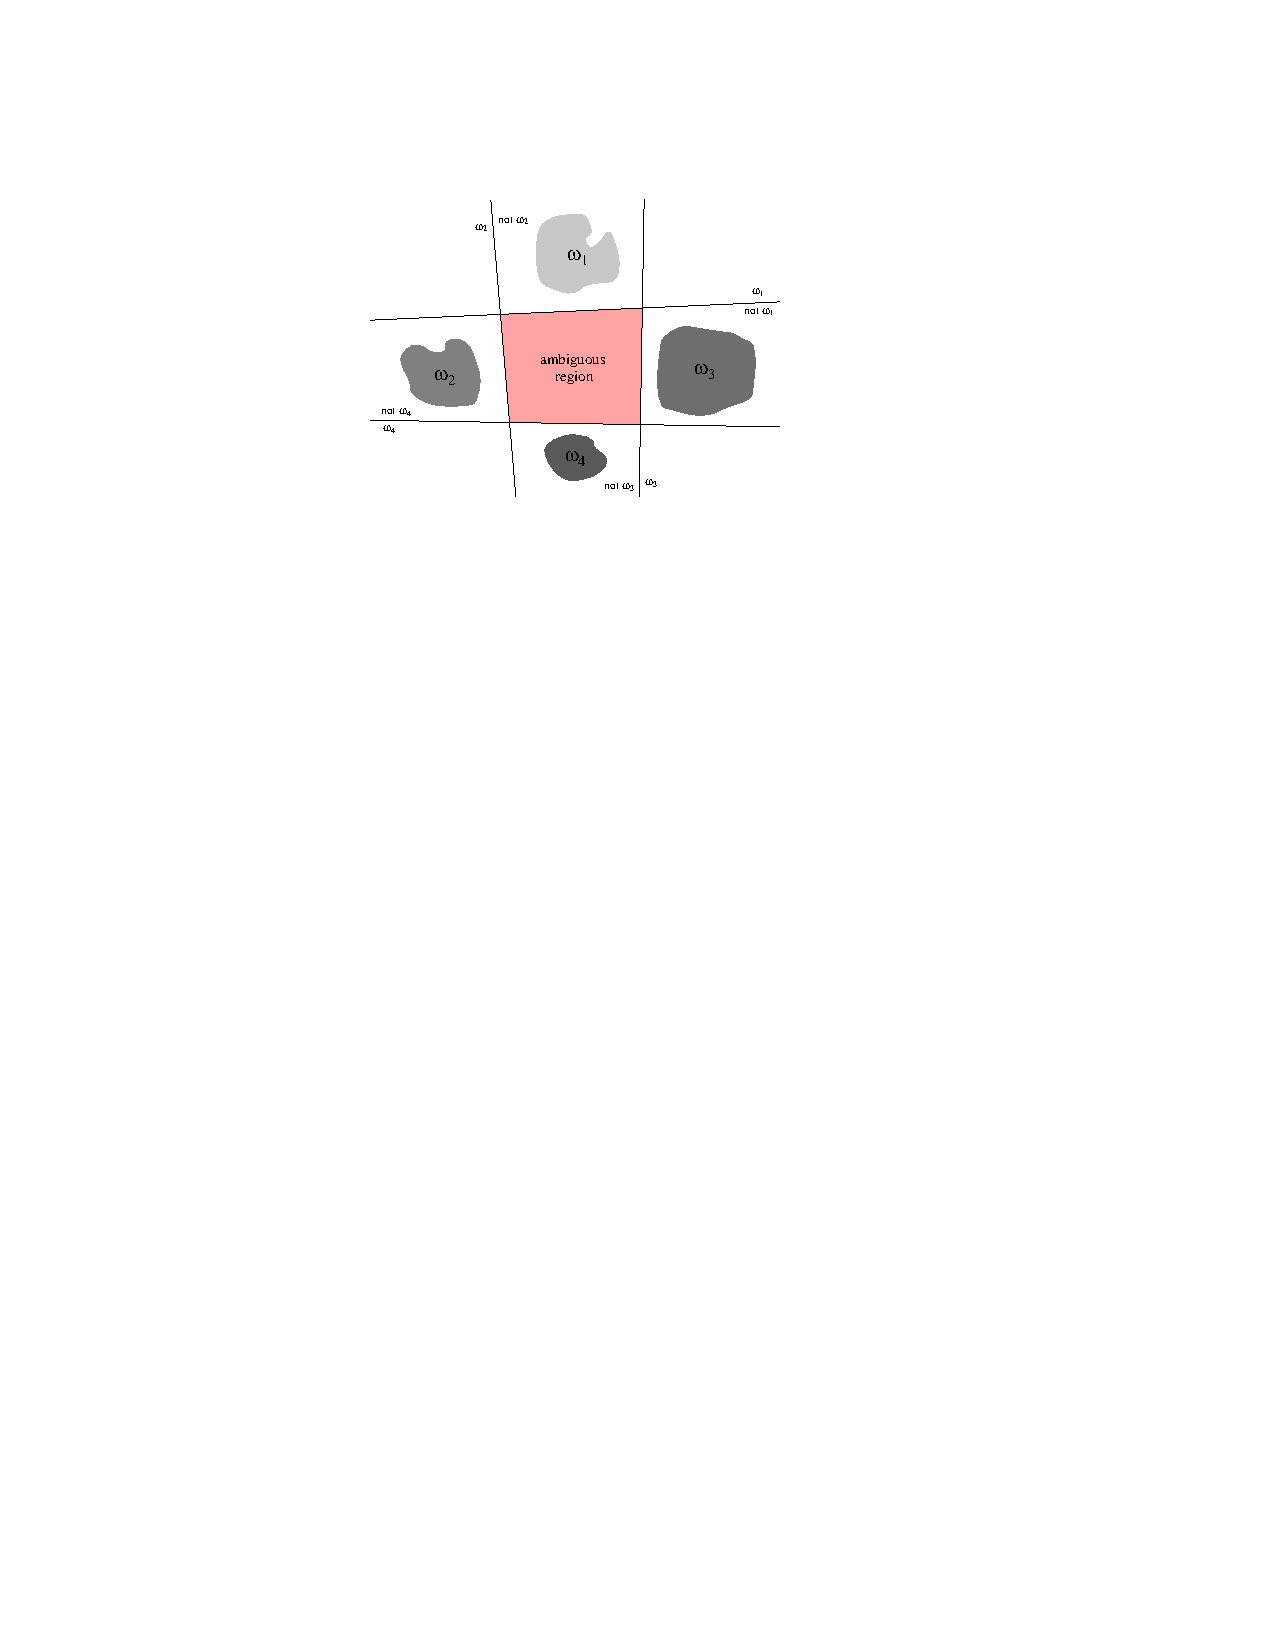
\includegraphics[scale=0.7]{ldf01}~~~~~~~
%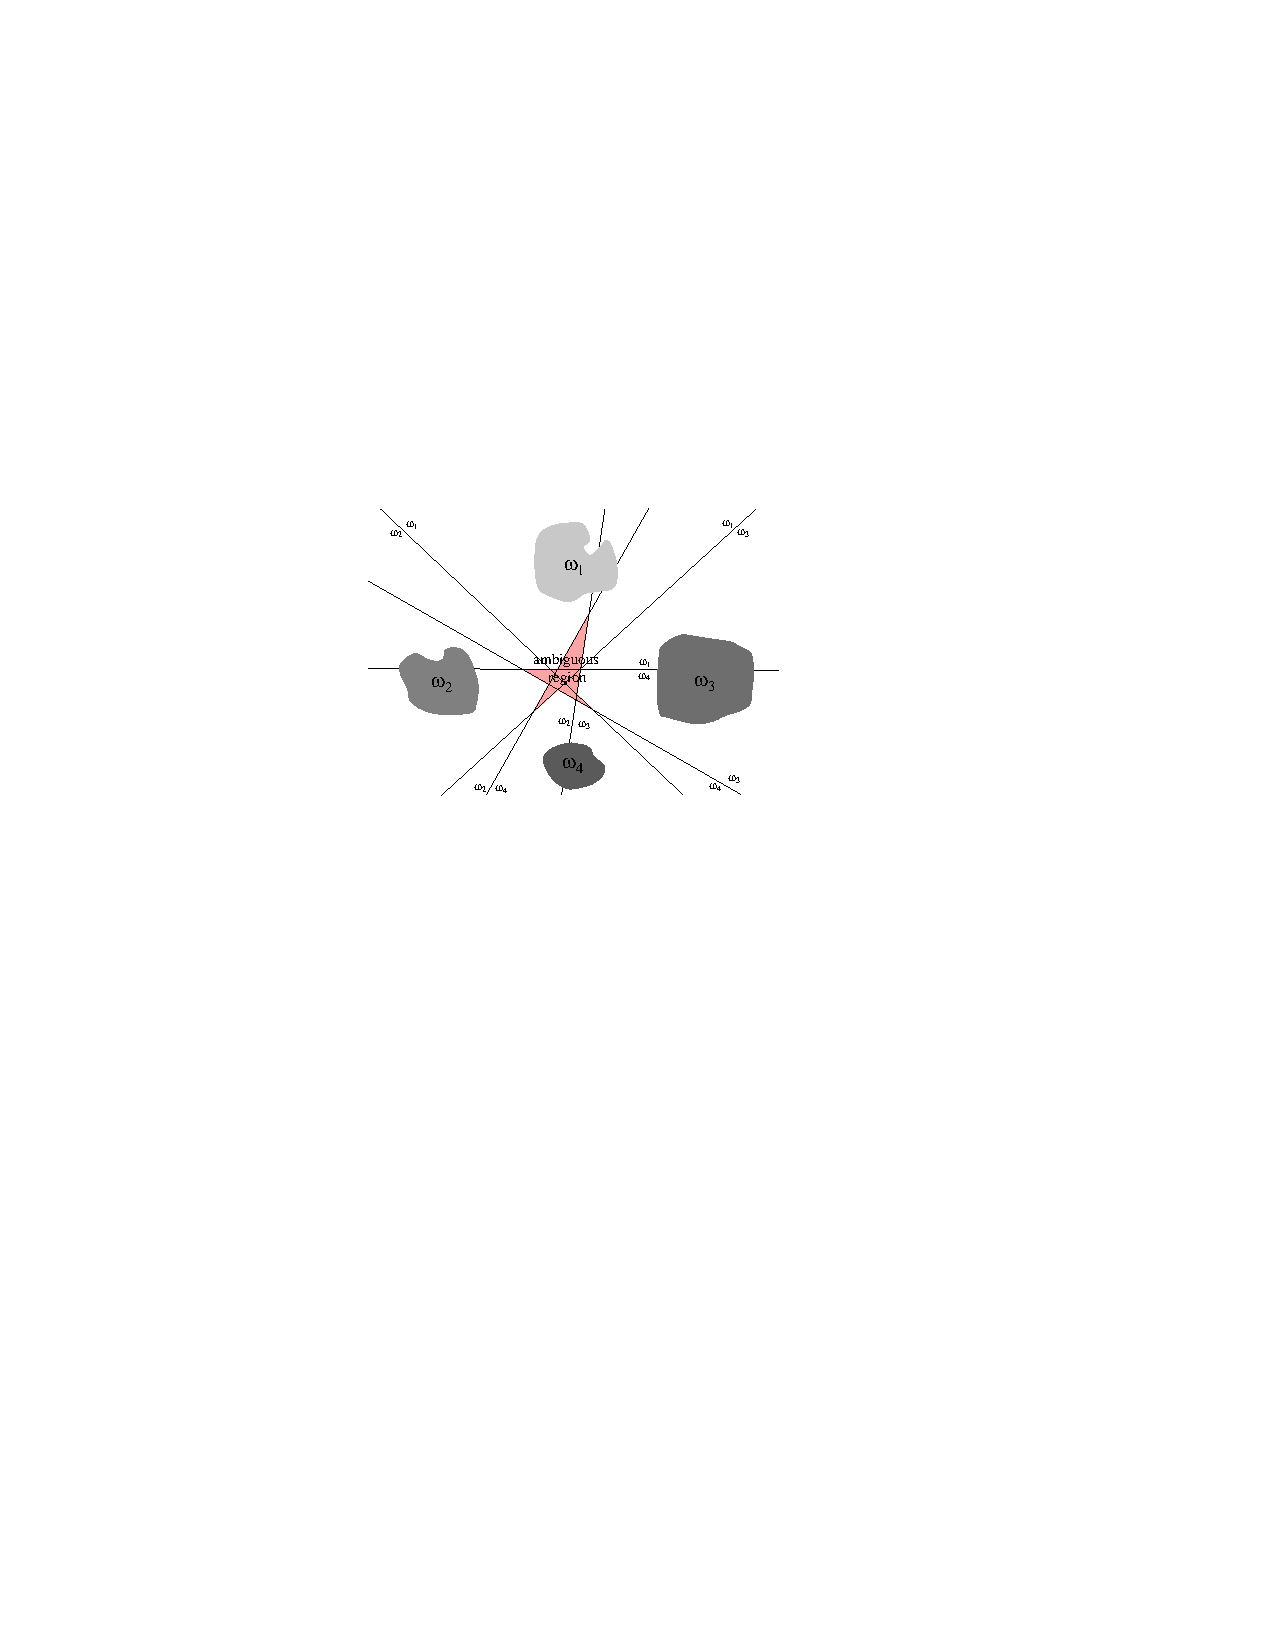
\includegraphics[scale=0.7]{ldf02}
%\caption{Linear decision boundaries fro a four-class problem devised as four two-class problems (left figure) and six pairwise problems (right figure). The pink regions have ambiguous category assignments.}
%\end{figure}
%\end{frame}

%\begin{frame}{The Multicategory Case}
%\begin{figure}
%\includegraphics[scale=0.8]{ldf03}
%\caption{Decision boundaries produced by a linear machine for a three-class problem and a five-class problem.}
%\end{figure}
%\end{frame}
\section{Generalized LDF}
\subsection{}

\begin{frame}{}
\begin{variableblock}{\centering \Large \textbf{\vspace{4pt}\newline Generalized Linear Discriminant Functions\vspace{4pt}}}{bg=slidecolor,fg=white}{bg=slidecolor,fg=white}
\end{variableblock}
\end{frame}
\begin{frame}{Generalized Linear Discriminant Functions}
\begin{itemize}
\item The linear discriminant function $g({\rm x})$ is defined as
\begin{align}
g({\rm x}) &= {\rm w}^T{\rm x}+w_0 \\
&= w_0+\sum_{i=1}^d w_ix_i
\end{align}
%\begin{figure}
%
\includegraphics[scale=1]{ldf04}
%\end{figure}
where ${\rm w}=[w_1,\ldots,w_d]^T$,  and ${\rm x}=[x_1,x_2,\ldots,x_d]^T$
\item We can obtain the \textit{\color{mycolor2}quadratic discriminant function} by adding second-order terms as
\begin{equation}
g({\rm x}) = w_0+\sum_{i=1}^d w_ix_i+\sum_{i=1}^d\sum_{j=1}^dw_{ij}x_ix_j
\end{equation}
%\begin{figure}
%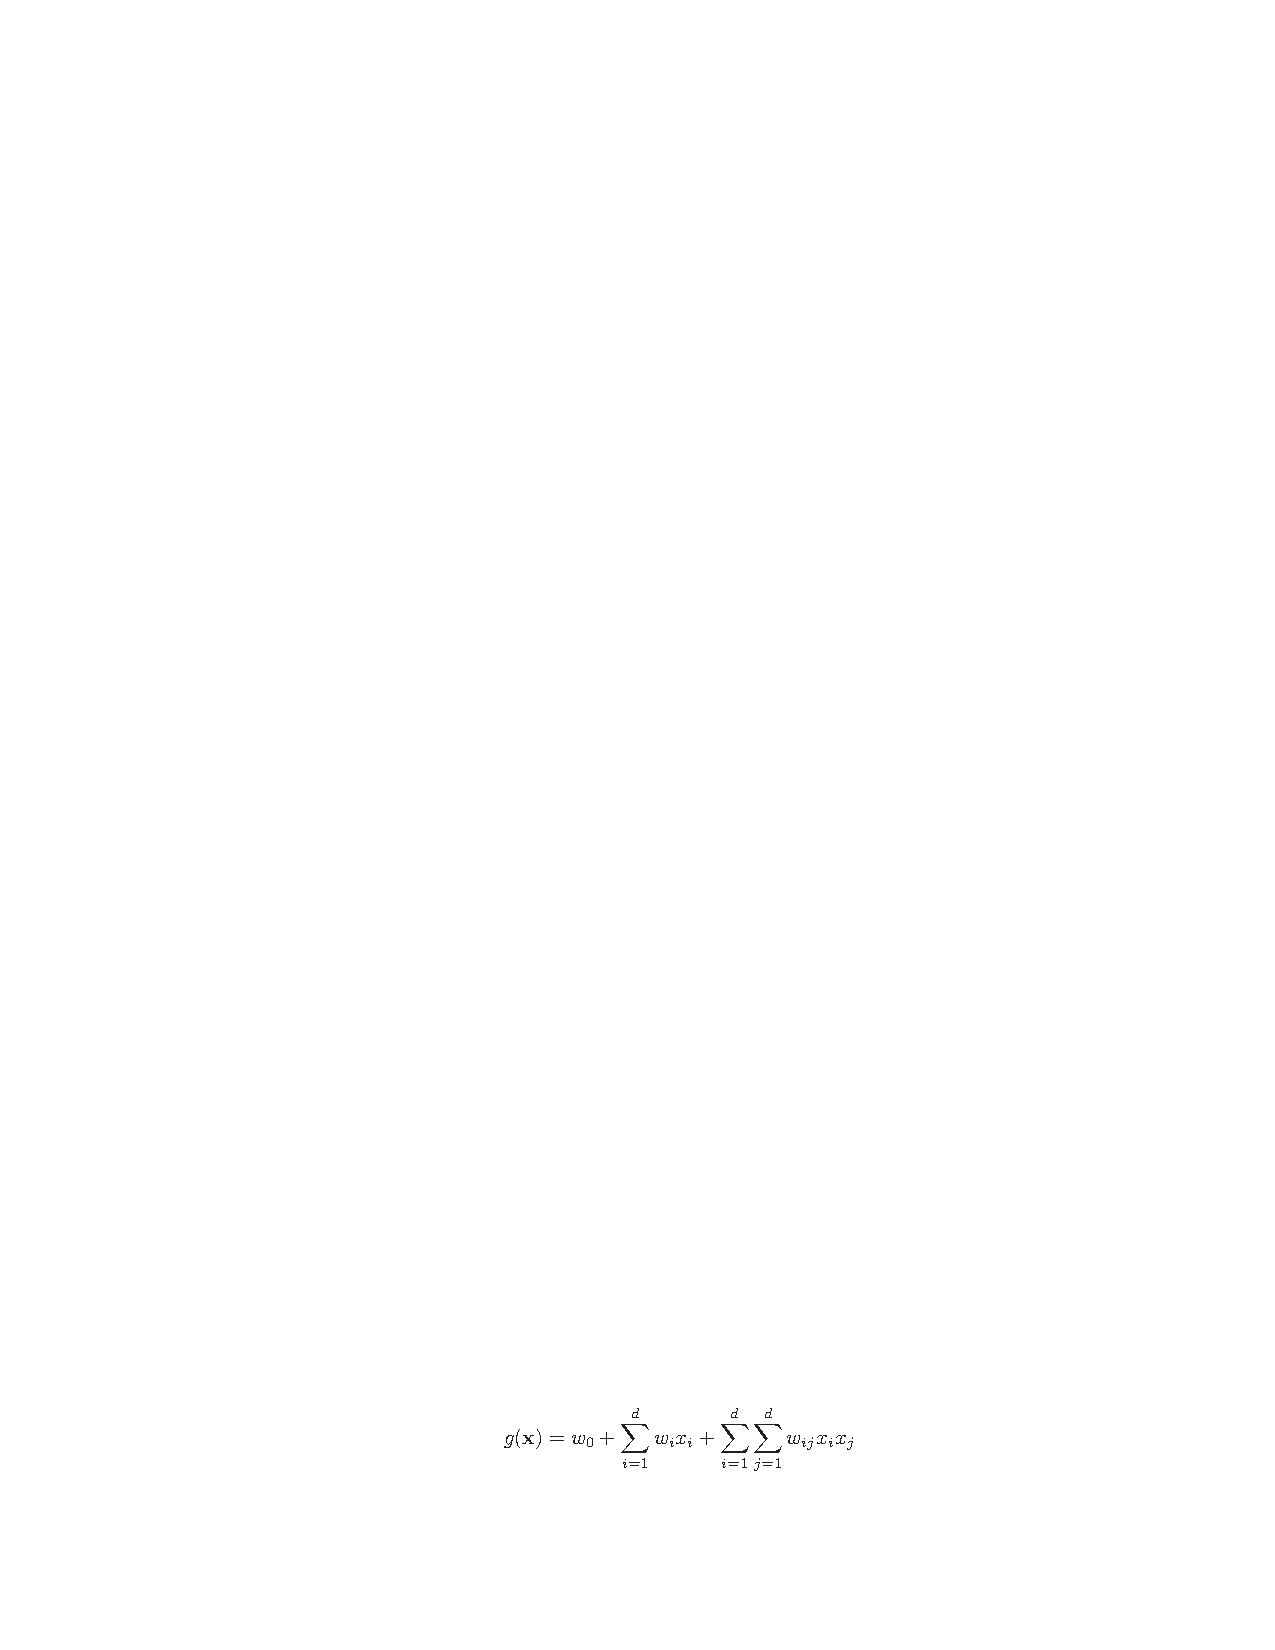
\includegraphics[scale=1]{ldf05}
%\end{figure}
Because $x_ix_j=x_jx_i$, we can assume that ${\rm w}_{ij}={\rm w}_{ji}$  with no loss in generality. Which result in more complicated decision boundaries.
({\color{mycolor2}hyperquadrics})
\end{itemize}
\end{frame}

\begin{frame}{Generalized Linear Discriminant Functions}
\begin{itemize}
\item The quadratic discriminant function has an additional $d(d+1)/2$ coefficients at its disposal with which to produce more complicated separating surfaces.
\item The separating surface defined by $g({\rm x})=0$ is a second-degree or hyperquadric surface.
\item If the symmetric matrix, ${\rm W} = [{\rm w}_{ij}]$, is nonsingular, the linear term in $g({\rm x})$ can be eliminated by translating the axes. 

\end{itemize}
\vspace{3cm}
\end{frame}

\begin{frame}{Generalized Linear Discriminant Functions}
\begin{itemize}
\item The basic character of the separating surface can be described in terms of scaled matrix
\begin{equation}
\bar{\rm W} = \frac{{\rm W}}{{{{\rm w}^T}{{\rm W}^{ - 1}}{\rm w} - 4{w_0}}} \nonumber
\end{equation}
where ${\rm w}=(w_1,\ldots,w_d)^T$ and ${\rm W}=[w_{ij}]$
\item The types of quadratic separating surfaces that arise in the general multivariate Gaussian case are as follows
\begin{itemize}
\item[1.] If $\bar{\rm W}$ is a positive multiple of the identity matrix, the separating surface is a \textit{\color{mycolor2}hypersphere} such that $\bar{\rm W}=kI$.
\item[2.] If $\bar{\rm W}$ is positive definite, the separating surfaces is a \textit{\color{mycolor3}hyperellipsoid} whose axes are in the direction of the eigenvectors of $\bar{\rm W}$.
\item[3.] If none of the above cases holds, that is, some of the eigenvalues of are positive and others are negative,
the surface is one of the varieties of types of \textit{\color{mycolor4}hyperhyperboloids}.
\end{itemize}
\end{itemize}
\end{frame}

\begin{frame}{Generalized Linear Discriminant Functions}
\begin{itemize}
\item By continuing to add terms such as $w_{ijk}x_ix_jx_k$, we can obtain the class of \textit{\color{mycolor2}polynomial discriminant functions}.
These can be thought of as truncated series expansions of some arbitrary $g ( {\rm x} )$, and this in turn suggest the
\textit{\color{mycolor2}generalized linear discriminant function}.
\begin{equation}
g({\rm x}) = \sum\limits_{i = 1}^{\hat d} {{a_i}{{\rm y}_i}({\rm x}) = {{\rm a}^T}{\rm y}} \nonumber
\end{equation}
where ${\rm a}$ is a $\hat{d}-$dimensional weight vector and $\hat{d}$ functions ${\rm y}_i({\rm x})$ are arbitrary functions of ${\rm x}$.
\item The physical interpretation is that the functions ${\rm y}_i({\rm x})$ map points ${\rm x}$ from $d$-dimensional space to point ${\rm y}$ in $\hat{d}$-dimensional space.
\item The resulting discriminant function is not linear in ${\rm x}$, but it is linear in ${\rm y}$.
\end{itemize}
\end{frame}

\begin{frame}{Generalized Linear Discriminant Functions}
\begin{itemize}
\item Then, the discriminant $g({\rm x}) = {\rm a}^T {\rm y}$ separates points in the transformed space using a hyperplane passing through the origin.
\item The mapping to a higher dimensional space may increase the complexity of the learning algorithms.
\item However, certain assumptions can make the problem tractable.
\item Let the quadratic discriminant function be
\begin{equation}
g({\rm x})=a_1+a_2{\rm x}+a_3{\rm x}^2 \nonumber
\end{equation}
\item So that the three-dimensional vector ${\rm y}$ is given by
\begin{equation}
{\rm y}=[1~~{\rm x}~~{\rm x}^2]^T \nonumber
\end{equation}
%\item {\color{mycolor1}Kernel trick} implicitly maps their input into high-dimensional feature space.
\end{itemize}
\end{frame}

\begin{frame}{Generalized Linear Discriminant Functions}
\begin{figure}
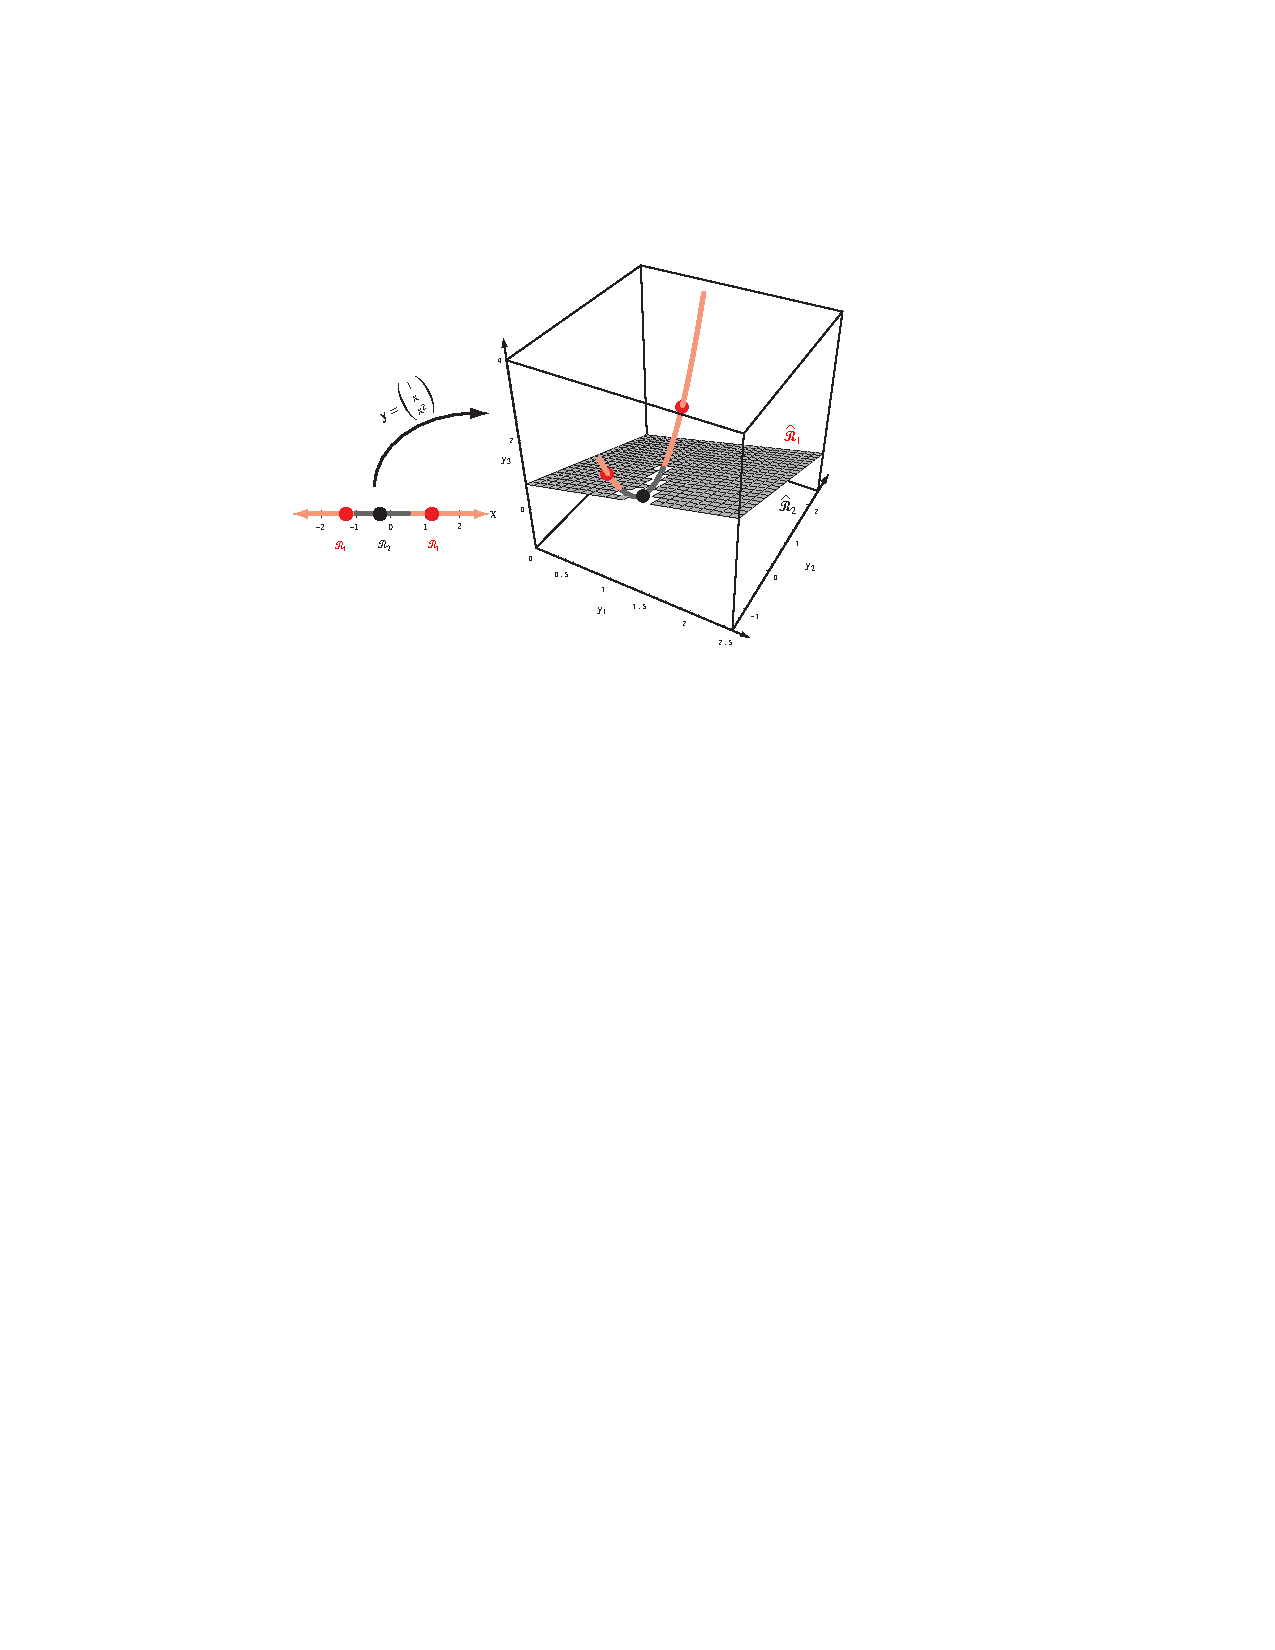
\includegraphics[scale=0.8]{ldf06}
\caption{The mapping ${\rm y} = (1~~ {\rm x}~~ {\rm x}^2 )^T$ takes a line and transforms it to a parabola
in three dimensions. A plane splits the resulting ${\rm y}$ space into regions corresponding
to two categories, and this in turn gives a non-simply connected decision region in the
one-dimensional ${\rm x}$ space.}
\end{figure}
\end{frame}

\begin{frame}{Generalized Linear Discriminant Functions}
\begin{figure}
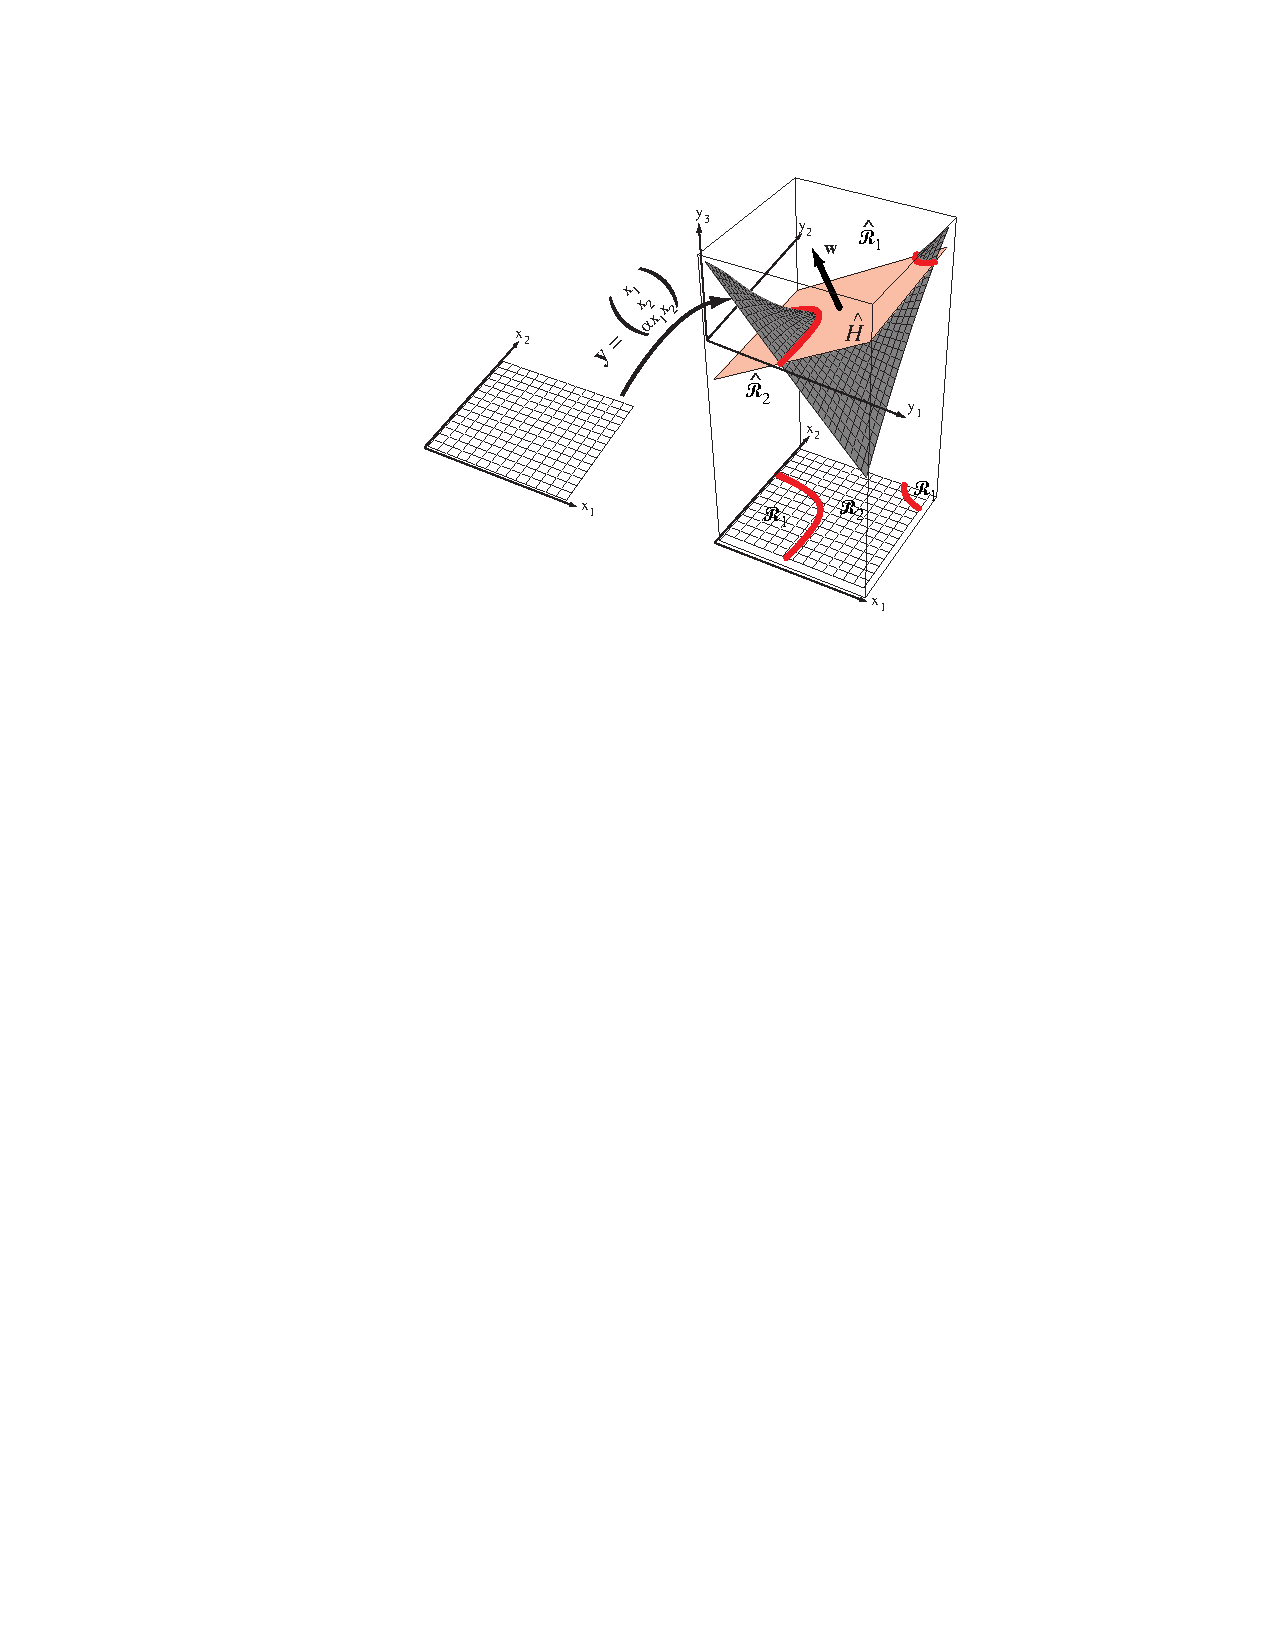
\includegraphics[scale=0.67]{ldf23}
\caption{The two-dimensional input space ${\rm x}$ is mapped through a polynomial
function $f$ to ${\rm y}$. Here the mapping is ${ y}_1 = {x}_1$ , ${y}_2 = {x}_2$ and ${y}_3\propto {x}_1 {x}_2$ . A linear
discriminant in this transformed space is a hyperplane, which cuts the surface. Points to the positive side of the hyperplane $\hat{H}$ correspond to category $\omega_1$ , and those beneath
it $\omega_2$. Here, in terms of the ${\rm x}$ space, $\mathcal{R}_1$ is a not simply connected.}
\end{figure}
\end{frame}

\begin{frame}{Problem to be solved}
\begin{small}
\textbf{\color{mycolor2}Question}:\\
The following three decision functions are given for a three-class problem.
\begin{align*}
g_1({\rm x}) &= 10x_1 -x_2 -10 = 0\\
g_2 ({\rm x}) &= x_1 + 2x_2 - 10 = 0\\
g_3({\rm x}) &= x_1 -2x_2 -10 = 0
\end{align*}
\begin{itemize}
\item[i.] Sketch the decision boundary and regions for each pattern class.
\item[ii.] Assuming that each pattern class is pairwise linearly separable from every other class
by a distinct decision surface and letting
\begin{align*}
g_{12}({\rm x}) &= g_1({\rm x})\\
g_{13}({\rm x}) &= g_2({\rm x})\\
g_{23}({\rm x}) &= g_3({\rm x})
\end{align*}
as listed above, sketch the decision boundary and regions for each pattern class.
\end{itemize}
\end{small}
\end{frame}

\section{Linearly separable case}
\subsection{}

\title{\fontsize{33}{45}{\huge Pattern Classification\newline{\large Lecture 06: Linear Discriminant Functions}\newline \vspace{8pt} \Large \vspace{-1.1cm}}}

\vspace{0.5cm}
\author{\vspace{0.4cm}\\\large{\bf Kundan Kumar\\\url{https://github.com/erkundanec/PatternClassification}}
%Associate Professor\\Department of ECE}
}
% - Give the names in the same order as the appear in the paper.
% - Use the \inst{?} command only if the authors have different
%   affiliation.
%\vspace{1cm}
\institute[Indian Institute of Technology Kharagpur] % (optional, but mostly needed)
{
\vspace{1.8cm}
%\includegraphics[height=.17\textheight]{SOAlogo.png}\\
% Faculty of Engineering (ITER)\\ S`O'A Deemed to be University, Bhubaneswar, India-751030\\


 \copyright\  2020 Kundan Kumar, All Rights Reserved\\
  \vspace{-1.1cm}}
% - Use the \inst command only if there are several affiliations.
% - Keep it simple, no one is interested in your street address.
\date{}
% To remove page number from a perticular slide
{
\setbeamertemplate{logo}{}
\makeatletter
\setbeamertemplate{footline}{
        \leavevmode%
  
  % First line.
  \hbox{%
  \begin{beamercolorbox}[wd=.2\paperwidth,ht=\beamer@decolines@lineup,dp=0pt]{}%
  \end{beamercolorbox}%
  \begin{beamercolorbox}[wd=.8\paperwidth,ht=\beamer@decolines@lineup,dp=0pt]{lineup}%
  \end{beamercolorbox}%
  } %
  % Second line.
  \hbox{%
  \begin{beamercolorbox}[wd=\paperwidth,ht=\beamer@decolines@linemid,dp=0pt]{linemid}%
  \end{beamercolorbox}%
  } %
  % Third line.
  \hbox{%
  \begin{beamercolorbox}[wd=.1\paperwidth,ht=\beamer@decolines@linebottom,dp=0pt]{}%
  \end{beamercolorbox}%
  \begin{beamercolorbox}[wd=.9\paperwidth,ht=\beamer@decolines@linebottom,dp=0pt]{linebottom}%
  \end{beamercolorbox}%
  }%
        }
\makeatother
\begin{frame}
\titlepage
\end{frame}
}



%\begin{frame}{Topics}
%\begin{itemize}
%%\item Linear Discriminant Functions and Decision Surfaces
%%\item Generalized Linear Discriminant Functions
%\item The two-category linearly separable case
%\item Perceptron Criterion Function
%\item Criterion Function
%\item Minimum Squared Error Procedures
%\item The Ho-Kashyap Procedures
%\end{itemize}
%\end{frame}

\begin{frame}{}
\begin{variableblock}{\centering \Large \textbf{\vspace{4pt}\newline Two-category linearly separable case\vspace{4pt}}}{bg=slidecolor,fg=white}{bg=slidecolor,fg=white}
\end{variableblock}
\end{frame}

\begin{frame}{2-category linearly separable case}
\begin{itemize}
\item Suppose, we have a set of $n$ samples ${\rm y}_1,\ldots,{\rm y}_n$
some labeled $\omega_1$ and some labeled $\omega_2$.
\item Note that all samples are augmented feature vectors.
\item We want to use these samples to determine the weights ${\rm a}$ in a linear discriminant function $g({\rm x}) = {\rm a}^T {\rm y}$.
\item If such ${\rm a}$ exists that
\begin{itemize}
\item ${\rm a}^T {\rm y}_i > 0$ for all ${\rm y}_i$ belonging to $\omega_1$, and
\item ${\rm a}^T {\rm y}_i < 0$ for all ${\rm y}_i$ belonging to $\omega_2$
\end{itemize}
samples ${\rm y}_1,\ldots,{\rm y}_n$ are called {\color{mycolor2}linearly separable}.
\item Then, it is reasonable to try to find such ${\rm a}$ that all the
training samples are classified correctly.
\end{itemize}
\end{frame}

\begin{frame}{2-category linearly separable case}
\begin{itemize}
\item {\color{mycolor1}Normalize the samples ${\rm y}_1,\ldots,{\rm y}_n$}: replace all ${\rm y}_i$ labeled $\omega_2$ by their negatives.
\begin{figure}
\includegraphics[scale=0.8]{LDF060}
\end{figure}
\item With this normalized set of training samples, we can
forget about labels and look for the weight vector ${\rm a}$ that
satisfies
\[{\rm a}^T{\rm y}_i > 0~~~~~~\text{       for all } {\rm y}_i.\]
\item Such ${\rm a}$ is called a {\color{mycolor2}solution vector}.
\end{itemize}
\end{frame}

\begin{frame}{Solution regions}
\begin{itemize}
\item A {\color{mycolor2}solution vector} - if exists - is not unique. The set of possible solution vectors, that are interpreted as points
in $\Re^d$, is called the {\color{mycolor4}solution region}.
\item More formally the solution region is the set
\[\left\{ {{\rm a} ~|~{{\rm a}^T}{{\rm y}_i} > 0;~~~~~\text{  for all  } i = 1, \ldots ,n} \right\}\]
\item There are several ways to impose additional requirements to constrain the solution vector. 
\item One possibility is to seek a unit-length weight vector that maximizes the minimum distance from the samples to the separating plane.

\end{itemize}
\end{frame}

\begin{frame}{Solution regions}
\begin{itemize}
\item Another possibility is to seek the minimum-length weight vector satisfying
\[{\rm a}^T {\rm y}_i \geq b,~~\forall~ i= 1,\ldots,n\]
where, $b$  is a positive constant, called the {\color{mycolor2}margin}.
\begin{figure}
\includegraphics[scale=0.75]{LDF071}
\end{figure}
\end{itemize}
\end{frame}

\begin{frame}{Solving inequalities}
\begin{itemize}
\item To find a solution to the set of linear inequalities
\[{\rm a}^T{\rm y}_i > 0\]
we define a criterion function $J({\rm a})$ that is minimized if ${\rm a}$ is a solution.
\item This kind of problem can be solved by {\color{mycolor2}gradient descent}.
\item The idea is very simple: Start with some vector ${\rm a}(1)$.
Generate then ${\rm a}(2)$ by taking a small step in the
direction of $-\nabla J({\rm a}(1))$ and so on.
\item Explanation: $-\nabla J({\rm a}(k))$ is the direction of the steepest descent.
\item In general, ${\rm a}(k + 1)$ is obtained from ${\rm a}(k)$ by the equation
\[{\rm a}(k + 1) = {\rm a}(k)-\eta (k)\nabla J({\rm a}(k)),\]
where $\eta$ is a positive scale factor or {\color{mycolor2}learning rate} that sets the step size.
\end{itemize}
\end{frame}

\begin{frame}{Basic gradient descent algorithm}
\begin{columns}
\begin{column}{7cm}
\vspace{-0.7cm}
\begin{figure}
\includegraphics[scale=1]{LDF073}
\end{figure}
\vspace{-0.5cm}
%\begin{itemize}
%\item[1.] Initialize: ${\rm a}(1)$, threshold $\theta$,learning rate $\eta(k)$, and set $k\leftarrow 0$.
%\item[2.] $k\leftarrow k + 1$
%\item[3.] ${\rm a}(k + 1) = {\rm a}(k)-\eta (k)\nabla J({\rm a}(k))$
%\item[4.] If $|\eta (k)\nabla J({\rm a}(k))|<\theta$ stop and return ${\rm a}(k)$, otherwise go to step 2.
%\end{itemize}
\onslide<2->{\begin{itemize}
\item The learning rate can be set
\[\eta (k) = \frac{{{{\left\| {\nabla J({\rm a}(k))} \right\|}^2}}}{{\nabla J{{({\rm a}(k))}^T}H\nabla J({\rm a}(k))}}\]
where $H$ is the Hessian at ${\rm a}(k)$.
\end{itemize}}
\end{column}
\begin{column}{7cm}
\vspace{-6pt}
\begin{figure}
\includegraphics[scale=0.4]{LDF072.png}
\end{figure}
\end{column}
\end{columns}
\end{frame}

\begin{frame}{Newton’s algorithm}
\begin{columns}
\begin{column}{7cm}
\begin{figure}
\includegraphics[scale=1]{LDF074}
\end{figure}
\end{column}
\begin{column}{7cm}
\begin{figure}
\includegraphics[scale=0.85]{LDF075}
\end{figure}
\end{column}
\end{columns}
\vspace{12pt}
\begin{itemize}
\item Another possibility is to set the learning rate to be a
constant that is small enough. This makes one iteration
of the descent algorithm much faster, but the descent
takes with a constant learning rate more iterations.
There is no general answer how to set the learning rate
optimally: The best selection depends on the
application.
\end{itemize}
\end{frame}


\section{Perceptron Criteria}
\subsection{}

\title{\fontsize{33}{45}{\huge Pattern Classification\newline{\large Lecture 06: Linear Discriminant Functions}\newline \vspace{8pt} \Large \vspace{-1.1cm}}}

\vspace{0.5cm}
\author{\vspace{0.4cm}\\\large{\bf Kundan Kumar\\\url{https://github.com/erkundanec/PatternClassification}}
%Associate Professor\\Department of ECE}
}
% - Give the names in the same order as the appear in the paper.
% - Use the \inst{?} command only if the authors have different
%   affiliation.
%\vspace{1cm}
\institute[Indian Institute of Technology Kharagpur] % (optional, but mostly needed)
{
\vspace{1.8cm}
%\includegraphics[height=.17\textheight]{SOAlogo.png}\\
% Faculty of Engineering (ITER)\\ S`O'A Deemed to be University, Bhubaneswar, India-751030\\


 \copyright\  2020 Kundan Kumar, All Rights Reserved\\
  \vspace{-1.1cm}}
% - Use the \inst command only if there are several affiliations.
% - Keep it simple, no one is interested in your street address.
\date{}
% To remove page number from a perticular slide
{
\setbeamertemplate{logo}{}
\makeatletter
\setbeamertemplate{footline}{
        \leavevmode%
  
  % First line.
  \hbox{%
  \begin{beamercolorbox}[wd=.2\paperwidth,ht=\beamer@decolines@lineup,dp=0pt]{}%
  \end{beamercolorbox}%
  \begin{beamercolorbox}[wd=.8\paperwidth,ht=\beamer@decolines@lineup,dp=0pt]{lineup}%
  \end{beamercolorbox}%
  } %
  % Second line.
  \hbox{%
  \begin{beamercolorbox}[wd=\paperwidth,ht=\beamer@decolines@linemid,dp=0pt]{linemid}%
  \end{beamercolorbox}%
  } %
  % Third line.
  \hbox{%
  \begin{beamercolorbox}[wd=.1\paperwidth,ht=\beamer@decolines@linebottom,dp=0pt]{}%
  \end{beamercolorbox}%
  \begin{beamercolorbox}[wd=.9\paperwidth,ht=\beamer@decolines@linebottom,dp=0pt]{linebottom}%
  \end{beamercolorbox}%
  }%
        }
\makeatother
\begin{frame}
\titlepage
\end{frame}
}



\begin{frame}{}
\begin{variableblock}{\centering \Large \textbf{\vspace{4pt}\newline Minimizing Perceptron Criterion Function\vspace{4pt}}}{bg=slidecolor,fg=white}{bg=slidecolor,fg=white}
\end{variableblock}
\end{frame}


\begin{frame}{Perceptron Criterion Function}
\begin{itemize}
\item Consider now the problem of {\color{mycolor2}constructing a criterion function} for solving the linear inequalities. Assume that
the margin $b = 0$.
\item The most obvious choice would be the {\color{mycolor2}number of
samples misclassified} by ${\rm  a}$. However, this criterion is a piece-wise constant function and a poor candidate for a gradient search.
\item The {\color{mycolor4}perceptron criterion function} is defined by
\[{J_p}({\rm a}) = \sum\limits_{{\rm y} \in \mathcal{Y}} { - {{\rm a}^T}{\rm y}}, \]
where $\mathcal{Y}$ is the set of samples misclassified by ${\rm a}$, i.e. samples for which the inner product with ${\rm a}$ is negative.
\end{itemize}
\end{frame}

\begin{frame}{Perceptron Criterion Function}
\begin{itemize}
\item The gradient
\[\nabla {J_p} = \sum\limits_{{\rm y} \in \mathcal{Y}} { - {{\rm y}}}, \]
\item The update rule in gradient descent is 
\[{{\rm a}}(k + 1) = {{\rm a}}(k) + \eta (k)\sum\limits_{{\rm y} \in \mathcal{Y}_k} {{\rm y}} \]
where $\mathcal{Y}_k$ is the set of samples misclassified by ${\rm a}(k)$.
\end{itemize}
\end{frame}

\begin{frame}{Perceptron Algorithm}
\begin{figure}
\includegraphics[scale=1,left]{LDF076}
\end{figure}
\vspace{-12pt}
\begin{itemize}
\item A good feature of the perceptron algorithm is that it will converge to a solution vector if training samples are linearly separable and the learning rate satisfies certain conditions.
\item A bad feature of the perceptron algorithm is that it does not (necessarily) converge if the training samples are not linearly separable.
\end{itemize}
\end{frame}

\begin{frame}{Other criterion functions}
\begin{itemize}
\item Relaxation Criterion:
\[{J_r}({\rm a}) = \frac{1}{2}\sum\limits_{y \in \mathcal{Y}} {\frac{{{{({{\rm a}^T}{\rm y} - b)}^2}}}{{{{\left\| {\rm y} \right\|}^2}}}} \]
where $b$ is the margin and $\mathcal{Y}({\rm a})$ is the set of samples for which ${\rm a}^T{\rm y}\leq b$.
\item Sum-of-squared-error criterion:
\[{J_s}({\rm a}) =||Y{\rm a}-b||^2= \sum\limits_{i = 1}^n {{{\left( {{{\rm a}^T}{{\rm y}_i} - b} \right)}^2}} \]
\end{itemize}
\end{frame}

\begin{frame}{Minimum Squared-Error and the Pseudoinverse}
\begin{itemize}
\item Let $Y$ be the $n\times \hat{d}$ matrix ($\hat{d}=d+1$), whose ith row is the vector ${\rm y}_i^T$.
\item Treat all linear equations simultaneously.
\[{\rm a}^T{\rm y}_i = {\rm b}~~~~~\forall i=1,\ldots,n\]
\item Combining all linear equation in a matrix form
\[\left[ {\begin{array}{*{20}{c}}
  {{y_{10}}}&{{y_{11}}}& \cdots &{{y_{1d}}} \\ 
  {{y_{20}}}&{{y_{21}}}& \cdots &{{y_{2d}}} \\ 
   \vdots & \vdots & \ddots & \vdots  \\ 
  {{y_{n0}}}&{{y_{n1}}}& \cdots &{{y_{nd}}} 
\end{array}} \right]\left[ {\begin{array}{*{20}{c}}
  {{a_0}} \\ 
  {{a_1}} \\ 
   \vdots  \\ 
  {{a_d}} 
\end{array}} \right] = \left[ {\begin{array}{*{20}{c}}
  {{b_1}} \\ 
  {{b_2}} \\ 
   \vdots  \\ 
  {{b_n}} 
\end{array}} \right]\]
\[\boxed{Y{\rm a}=b}\]
\end{itemize}
\end{frame}

\begin{frame}{Minimum Squared-Error and the Pseudoinverse}
\vspace{-4pt}
\begin{footnotesize}
\begin{itemize}
\item We seek for a weight vector ${\rm a}$ that minimizes some function of the error between $Y{\rm a}$ and ${\rm b}$.
\[{\rm e}=Y{\rm a}-{\rm b}\]
\item Sum-of-squared-error (SSE) criterion function:
\[{J_s}({\rm a}) =||Y{\rm a}-b||^2= \sum\limits_{i = 1}^n {{{\left( {{{\rm a}^T}{{\rm y}_i} - b} \right)}^2}} \]
\item Minimizing the criterion function
\begin{align*}
  \nabla {J_s} = \sum\limits_{i = 1}^n {2({{\rm a}^T}{{\rm y}_i} - {{\rm b}_i}){{\rm y}_i}}  = 2{Y^T}(Y{\rm a} - {\rm b}) =0 
\end{align*}
\begin{align*}
  Y^TY{\rm a}&=Y^T{\rm b}\\
  {\rm a} &= (Y^TY)^{-1}Y^T{\rm b} \\
  {\rm a} &=Y^{\dagger} {\rm b}
\end{align*}
\item However, $Y^{\dagger}$ is defined more generally by $\boxed{Y^{\dagger}\equiv \mathop {\lim }\limits_{\varepsilon  \to 0} {({Y^T}Y + \varepsilon I)^{ - 1}}{Y^T}}$
\end{itemize}
\end{footnotesize}
\end{frame}
\begin{frame}{Example}

{\color{mycolor2}Question:}

Suppose we have the following two-dimensional point for two categories: $\omega_1$: $(1,2)^T$ and $(2,0)^T$, and $\omega_2$: $(3,1)^T$ and $(2,3)^T$. Construct a Linear Classifier by Matrix Pseudoinverse.
\begin{figure}
\includegraphics[scale=0.8]{LDF077}
\end{figure}
\end{frame}


\section{References}
\subsection{}
\begin{frame}[allowframebreaks]{References}
\linespread{1}
\footnotesize
\printbibliography[heading=none]
\end{frame}
{
\setbeamertemplate{logo}{}
\makeatletter
\setbeamertemplate{footline}{
        \leavevmode%
  
  % First line.
  \hbox{%
  \begin{beamercolorbox}[wd=.2\paperwidth,ht=\beamer@decolines@lineup,dp=0pt]{}%
  \end{beamercolorbox}%
  \begin{beamercolorbox}[wd=.8\paperwidth,ht=\beamer@decolines@lineup,dp=0pt]{lineup}%
  \end{beamercolorbox}%
  } %
  % Second line.
  \hbox{%
  \begin{beamercolorbox}[wd=\paperwidth,ht=\beamer@decolines@linemid,dp=0pt]{linemid}%
  \end{beamercolorbox}%
  } %
  % Third line.
  \hbox{%
  \begin{beamercolorbox}[wd=.1\paperwidth,ht=\beamer@decolines@linebottom,dp=0pt]{}%
  \end{beamercolorbox}%
  \begin{beamercolorbox}[wd=.9\paperwidth,ht=\beamer@decolines@linebottom,dp=0pt]{linebottom}%
  \end{beamercolorbox}%
  }%
        }
\makeatother

\begin{frame}
\centering
\includegraphics[width=0.34\paperwidth]{queries.jpg}\\
\includegraphics[width=0.45\paperwidth]{thank_you.png}
\end{frame}
}
